\section{Computing cost bounds}

The last two chapters introduced algorithms for the computation of time bounds and size bounds.
The algorithm for the computation of time bounds uses the so far computed size bounds and the algorithm for the computation of size bounds uses the so far computed time bounds.
This chapter presents a cost bound algorithm, which runs after the consecutive executions of the time and size bound algorithms and uses the resulting time and size bounds for the computation of cost bounds.

\subsection{Computing trivial cost bounds}

A trivial approach for the computation of a cost bound $\UCost(t)$ of a transition $t \in \TSet$ is the multiplication of the time bound $\UTime(t)$ with the maximum of the substituted costs $\usubst{\cost(t)}{\LSize(\pret)}{\USize(\pret)}$ for a pre-transition $\pret \in \pre(t)$.
For the computation of a cost bound $\UCost(t)$ of an initial transition $t \in \TSet_0$ the substitution is not necessary, since there are no pre-transitions of an initial transition $t \in \TSet_0$ and the variables of the costs $\cost(t)$ are already expressed in dependence on the input variables of the program.

\begin{definition}[Trivial Cost Bound]
  Let $\UCost: \TSet \rightarrow \BoundSet(\PVSet)$ be defined with
  \[ \UCost(t) = \UTime(t) \cdot
  \begin{cases}
    \cost(t) & \text{if } t \in \TSet_0 \\
    \maximum{\usubst{\cost(t)}{\LSize(\pret)}{\USize(\pret)} \mid \pret \in \pre(t)} & \text{otherwise }
  \end{cases}
  \]
  Then, we call $\UCost$ a \textbf{trivial cost bound}. 
\end{definition}

Since the cost $\exacteval{\cost(t)}{\valuation}$ of a single evaluation step with $t \in \TSet$ is defined to be positive for every state $\valuation$, it is not necessary to use an operator $\maxO{\cdot}$ on the cost of a transition.

\begin{example}[Trivial cost bound]
  Consider the program in Figure \ref{fig:cost_ranking_function}.
  \begin{figure}
\centering

\begin{tikzpicture}[->,>=stealth',auto,node distance=5cm,
    thick,
    main node/.style={circle,draw,font=\sffamily\Large\bfseries},
    aligned edge/.style={align=left}]

  \node[main node] (0) {$\location_0$};
  \node[main node] (1) [right of=0] {$\location_1$};

  \path[every node/.style={font=\sffamily\small}]
    (0) edge[aligned edge] node[above=0.2cm] {$t_0$} node[below=0.2cm] {$\update = \emph{id}$} (1)
    (1) edge[aligned edge, loop above] node[left=0.2cm] {$t_1$} node[below right=0cm and 0.5cm] {$\update(x) = x - y$\\$\update(y) = y$\\$\guard = \braced{y > 0, x > y}$\\$\cost(t_1)=y$} (1)
    ;
\end{tikzpicture}

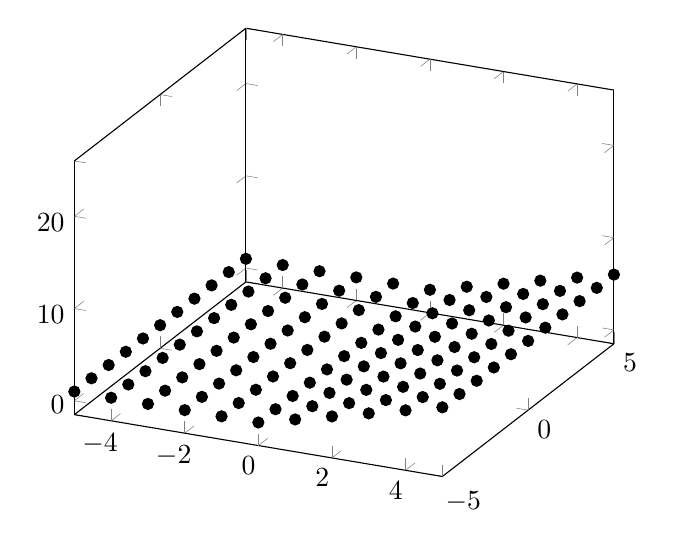
\begin{tikzpicture}
  \begin{axis}[zmax=26]
    \addplot3 [
      unbounded coords=jump,
      mesh,
      shader=interp,
      samples at={-5,...,5},
      samples y={11},
      only marks,
    ] {1+max(x,0)};
  \end{axis}
\end{tikzpicture}
\hfil
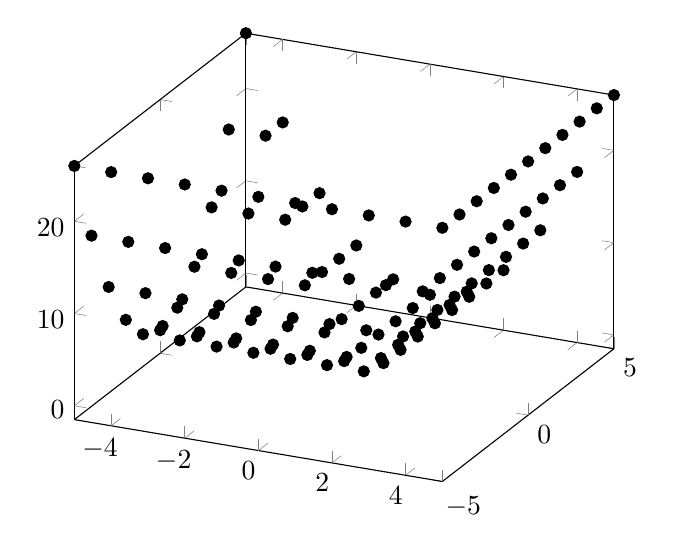
\begin{tikzpicture}
  \begin{axis}[zmax=26]
    \addplot3 [
      unbounded coords=jump,
      mesh,
      shader=interp,
      samples at={-5,...,5},
      samples y={11},
      only marks,
    ] {1+abs(max(x,-y))*abs(max(x,-y))};
  \end{axis}
\end{tikzpicture}

\caption{Evaluation of an example with cost ranking functions yielding a benefit}
\label{fig:cost_ranking_function}
\end{figure}

  The program takes two variables $x$ and $y$.
  It decreases the value of $x$ in each step with $t_1$ with the value of $y$.
  Each step with $t_1$ has a cost of the current value of $y$.
  Since the value of $y$ never changes, the cost of the transition $t_1$ is constant throughout the execution of the loop.
  The guard ensures that $x > y > 0$.
  Therefore, the method TimeBounds can compute a time bound $\UTime(t_1) = \maxO{x}$.
  Since the size of $y$ is bound with $\USize(t_0) = y$ after the transition $t_0$, a trivial cost bound $\UCost(t_1) = \UTime(t_1) \cdot \usubst{\cost(t_1)}{\LSize(t_0)}{\USize(t_0)} = \maxO{x} \cdot y$ can be inferred.
\end{example}

\subsection{Computing cost bounds with ranking functions}

Additionally to trivial cost bounds, we use ranking functions, to infer better cost bounds for single transitions.
With some changes the definition of time ranking functions is transferable to the context of costs.

\begin{definition}[Cost Ranking Function] 
  We define $\costrank: \LSet \rightarrow \BoundSet_p(\PVSet)$ as cost ranking function for a transition set $\TSet$ if and only if there is a nonempty set of strictly decreasing transitions $\TSet_{>} \subseteq \TSet$ such that the following statements hold.
  For all transitions $t = (\location, \update, \guard, \location') \in \TSet$ and every evaluation step $(\location, \valuation) \rightarrow_t (\location', \valuation')$ it holds that
  \[ \exacteval{\guard}{\valuation} \Rightarrow \exacteval{\costrank(\location)}{\valuation} \geq \exacteval{\costrank(\location')}{\valuation'}. \]
  For all transitions $(\location, \update, \guard, \location') \in \TSet_{>}$ and every evaluation step $(\location, \valuation) \rightarrow_t (\location', \valuation')$ it holds that        
  \[ \exacteval{\guard}{\valuation} \Rightarrow \exacteval{\costrank(\location)}{\valuation} - \exacteval{\cost(t)}{\valuation} \geq \exacteval{\costrank(\location')}{\valuation'} \]
  and
  \[ \exacteval{\guard}{\valuation} \Rightarrow \exacteval{\costrank(\location)}{\valuation} \geq \exacteval{\cost(t)}{\valuation} \]
\end{definition}

This definition ensures that each transition $t \in \TSet_>$ decreases in each transition step by its cost.
Also, for each transition $t \in \TSet_>$ the decrease of the rank  is bounded by the costs.
Therefore, the cost rank $\costrank(\location)$ can be used as a bound on the sum of all occurred costs of the transition $t$ from this location on.

\begin{example}[Cost ranking function]
  Consider again the program in Figure \ref{fig:cost_ranking_function}.
  We can show that the function $\costrank$ with $\costrank(\location_1) = x$ is a cost ranking function for the transition set $\TSet = \braced{t_1}$.
  For every evaluation step $(\location_1,\valuation) \rightarrow_{t_1} (\location_1,\valuation')$ it holds that $\exacteval{\braced{y > 0, x > y}}{\valuation} \Rightarrow \exacteval{x}{\valuation} - \exacteval{y}{\valuation} > \exacteval{x}{\valuation'}$, since the value of $x$ decreases in every evaluation step with the value of $y$.
  Also, it holds for every evaluation step $(\location_1,\valuation) \rightarrow_{t_1} (\location_1,\valuation')$ that $\exacteval{\braced{y > 0, x > y}}{\valuation} \Rightarrow \exacteval{x}{\valuation} \geq \exacteval{y}{\valuation}$, since the value of $x$ is greater than $y$ in every evaluation step.
\end{example}

With a few changes, the TimeBounds algorithm is extendable to the computation of cost bounds.

We want to prove the following claim for all transitions $t \in \TSet$ and all states $\lstate, \ustate \in \Valuation$.
\begin{align*}
  \ueval{\UCost'(t)}{\lstate}{\ustate} \geq \sup & \braced{ \sum_{1 \leq i \leq k} \exacteval{\cost(t)}{\valuation_i} \mid \exists \valuation_0, k \geq 1: \lstate \leq \valuation_0 \leq \ustate \\
    & \wedge (\location_0, \valuation_0) \rightarrow^* (\location_1, \valuation_1) (\rightarrow_t \circ \rightarrow^*) \dots (\location_k, \valuation_k) (\rightarrow_t \circ \rightarrow^*) (\location_{k+1}, \valuation_{k+1}) }
\end{align*}

This is trivial, if $t \notin \TSet'_>$.
Therefore, lets consider a transition $t \in \TSet'_>$.
It suffices to show that for all transitions $t \in \TSet'_>$ and all states $\lstate \leq \ustate$ the following claim holds.
\begin{align*}
  & \sum_{\location \in \mathcal{E}_{\TSet'}} \sum_{\pret \in \TSet_\location} \ueval{\UTime(\pret)}{\lstate}{\ustate} \cdot \maxO{\usubst{\costrank(\location)}{\leval{\LSize(\pret)}{\lstate}{\ustate}}{\ueval{\USize(\pret)}{\lstate}{\ustate}}} \\
  \geq \sup & \braced{ \sum_{1 \leq i \leq k} \exacteval{\cost(t)}{\valuation_i} \mid \exists \valuation_0, k \geq 1: \lstate \leq \valuation_0 \leq \ustate \\
    & \wedge (\location_0, \valuation_0) \rightarrow^* (\location_1, \valuation_1) (\rightarrow_t \circ \rightarrow^*) \dots (\location_k, \valuation_k) (\rightarrow_t \circ \rightarrow^*) (\location_{k+1}, \valuation_{k+1}) }
\end{align*}
To this end, let $\valuation_0$ be an initial state with $\lstate \leq \valuation_0 \leq \ustate$ and consider a (finite or infinite) evaluation starting with $\valuation_0$ where $k \in \mathbb{N} \cup \braced{\infty}$ steps are performed with the transition $t$.
The goal is now to show that
\[
  \sum_{\location \in \mathcal{E}_{\TSet'}} \sum_{\pret \in \TSet_\location} \ueval{\UTime(\pret)}{\lstate}{\ustate} \cdot \maxO{\usubst{\costrank(\location)}{\leval{\LSize(\pret)}{\lstate}{\ustate}}{\ueval{\USize(\pret)}{\lstate}{\ustate}}} \geq \sum_{1 \leq i \leq k} \exacteval{\cost(t)}{\valuation_i}
\]

This is trivial for $k = 0$.
Then it holds that $\sum_{1 \leq i \leq k} \exacteval{\cost(t)}{\valuation_i} = 0$.
Since the operator $\maxO{\cdot}$ ensures positivity and $\exacteval{\UTime(t)}{\valuation_0} \geq 0$ holds for any transition $t$, the statement holds.

We now consider the case $k > 0$.
Then, we can use the following representation for the considered evaluation.
\begin{IEEEeqnarray*}{lClClClCl}
  (\prel_0, \prestate_0) & \rightarrow^{\tilde{k}_0}_{\TSet \setminus \TSet'} & (\actl_{1,1}, \actstate_{1,1}) & \rightarrow_{\TSet'} & \dots & \rightarrow_{\TSet'} & (\actl_{1,k_1}, \actstate_{1,k_1}) & \rightarrow_{\TSet'} \\
  (\prel_1, \prestate_1) & \rightarrow^{\tilde{k}_1}_{\TSet \setminus \TSet'} & (\actl_{2,1}, \actstate_{2,1}) & \rightarrow_{\TSet'} & \dots & \rightarrow_{\TSet'} & (\actl_{2,k_2}, \actstate_{2,k_2}) & \rightarrow_{\TSet'} \\
  (\prel_2, \prestate_2) & \rightarrow^{\tilde{k}_2}_{\TSet \setminus \TSet'} & \dots
\end{IEEEeqnarray*}
In this evaluation, the outgoing transitions of all $(\actl_{i,h}, \actstate_{i,h})$ are transitions from $\TSet'$.
The outgoing transitions of all $(\prel_i, \prestate_i)$ are transitions from $\TSet \setminus \TSet'$.

Now we have to investigate how often the transition $t$ is used in this evaluation.
Since $t \in \TSet'$, it can only be used in sequences of the following form.
\[ (\actl_{i,1}, \actstate_{i,1}) \rightarrow_{\TSet'} \dots \rightarrow_{\TSet'} (\actl_{i,k_i}, \actstate_{i,k_i}) \rightarrow_{\TSet'} (\prel_i, \prestate_i) \]

We can show that $\maxO{\exacteval{\costrank(\location_{i,1})}{\actstate_{i,1}}} \geq \sum_{1 \leq h \leq {k_i}} \exacteval{\cost(t)}{\valuation_{i,h}}$.
For $k_i = 0$ this is obvious, since then $\sum_{1 \leq h \leq {k_i}} \exacteval{\cost(t)}{\valuation_{i,h}} = 0$ holds and the operator $\maxO{\cdot}$ ensures positivity.
Lets consider the case $k_i > 0$.
Since $\costrank$ is a cost ranking function for $\TSet'$, for all $j$ it holds that $\exacteval{\costrank(\location_{i,j})}{\actstate_{i,j}} \geq \exacteval{\costrank(\location_{i,j+1})}{\actstate_{i,j+1}}$.
Let $j_1 < j_2 < \dots$ be the indices where $t_j = t$.
Then, for all $j \in \braced{j_1, j_2, \dots}$, $t \in \TSet_>$ implies that $\exacteval{\costrank(\location_{i,j})}{\actstate_{i,j}} \geq \exacteval{\costrank(\location_{i,j+1})}{\actstate_{i,j+1}} + \exacteval{\cost(t)}{\actstate_{i,j}}$ and $\exacteval{\costrank(\location_{i,j})}{\actstate_{i,j}} \geq \exacteval{\cost(t)}{\actstate_{i,j}}$.
Thus, we obtain
\begin{align*}
  & \exacteval{\costrank(\location_{i,1})}{\actstate_{i,1}} \\
  \geq & \exacteval{\costrank(\location_{i,j_1})}{\actstate_{i,j_1}} \\
  \geq & \exacteval{\costrank(\location_{i,j_2})}{\actstate_{i,j_2}} + \exacteval{\cost(t)}{\actstate_{i,j_1}} \\
  \geq & \dots \\
  \geq & \exacteval{\costrank(\location_{i,j_{k_i}})}{\actstate_{i,j_{k_i}}} + \exacteval{\cost(t)}{\actstate_{i,j_{k_i-1}}} \\
  \geq & \exacteval{\cost(t)}{\actstate_{i,j_{k_i}}}
\end{align*}
Therefore, $\maxO{\exacteval{\costrank(\location_{i,1})}{\actstate_{i,1}}} \geq \sum_{1 \leq h \leq {k_i}} \exacteval{\cost(t)}{\valuation_{i,h}}$ is an upper bound on the costs of the transition $t$ in the sequence.

Let $\pret_i$ be the transition reaching $(\actl_{i,1}, \actstate_{i,1})$ in the evaluation.
Thus, we have $\actl_{i,1} \in \mathcal{E}_{\TSet'}$ and $\pret_i \in \TSet_{\actl_{i,1}}$.
As $(\location_0, \valuation_0) \rightarrow^*_\TSet \circ \rightarrow_{\pret_i} (\actl_{i,1}, \actstate_{i,1})$ and $\lstate \leq \valuation_0 \leq \ustate$, we have by definition of size bounds
\[ \ueval{\USize(\pret_i, v)}{\lstate}{\ustate} \geq \exacteval{\USize(\pret_i, v)}{\valuation_0} \geq \actstate_{i,1}(v) \geq \exacteval{\LSize(\pret_i, v)}{\valuation_0} \geq \leval{\LSize(\pret_i, v)}{\lstate}{\ustate}. \]
We can conclude
\begin{align*}
   & \maxO{\ueval{\costrank(\actl_{i,1})}{\leval{\LSize(\pret_i)}{\lstate}{\ustate}}{\ueval{\USize(\pret_i)}{\lstate}{\ustate}}} \\
   \geq & \maxO{\ueval{\costrank(\actl_{i,1})}{\exacteval{\LSize(\pret_i)}{\valuation_0}}{\exacteval{\USize(\pret_i)}{\valuation_0}}} \\
   \geq & \maxO{\ueval{\costrank(\actl_{i,1})}{\valuation_{i,1}}{\valuation_{i,1}}} \\
   \geq & \maxO{\exacteval{\costrank(\actl_{i,1})}{\valuation_{i,1}}} \\
   \geq & \sum_{1 \leq h \leq {k_i}} \exacteval{\cost(t)}{\valuation_{i,h}} \\
\end{align*}
Thus, $\maxO{\usubst{\costrank(\actl_{i,1})}{\leval{\LSize(\pret_i)}{\lstate}{\ustate}}{\ueval{\USize(\pret_i)}{\lstate}{\ustate}}}$ is a bound on the cost $\sum_{1 \leq h \leq {k_i}} \exacteval{\cost(t)}{\valuation_{i,h}}$ of the transition $t$ in the sequence.

It remains to examine how often a sequence $(\actl_{i,1}, \actstate_{i,1}) \rightarrow^*_{\TSet'} (\prel_i, \prestate_i)$ can occur in the full evaluation.
As observed earlier, the transition reaching $(\actl_{i,1}, \actstate_{i,1})$ in the evaluation is always some $\pret_i \in \TSet_{\actl_{i,1}}$.
Each $\pret_i$ can occur at most $\ueval{\UTime(\pret_i)}{\lstate}{\ustate}$ times in evaluations.
We found out, that in every $\TSet'$-sequence the transition $t$ has costs of at most $\maxO{\ueval{\costrank(\actl_{i,1})}{\leval{\LSize(\pret_i)}{\lstate}{\ustate}}{\ueval{\USize(\pret_i)}{\lstate}{\ustate}}}$.
Thus, we can infer that our initial statement holds.
\begin{IEEEeqnarray*}{rCl}
  \sum_{\location \in \mathcal{E}_{\TSet'}} \sum_{\pret \in \TSet_\location} \ueval{\UTime(\pret)}{\lstate}{\ustate} \cdot \maxO{\usubst{\costrank(\location)}{\leval{\LSize(\pret)}{\lstate}{\ustate}}{\ueval{\USize(\pret)}{\lstate}{\ustate}}} \geq \sum_{1 \leq i \leq k} \exacteval{\cost(t)}{\valuation_i}
\end{IEEEeqnarray*}


With this definition, it is possible to start with a trivial cost bound, search for cost ranking functions and consecutively refine the cost bounds of single transitions, where a cost ranking function is found.

\begin{example}[CostBounds]
  Consider again the program in Figure \ref{fig:cost_ranking_function}.
  We showed that a trivial cost bound can be computed as $\UCost(t_1) = \maxO{x} \cdot y$ and that a cost ranking function $\costrank$ with $\costrank(\location_1) = x$ can be determined.
  The resulting cost bound of the CostBounds method is $\UCost(t_1) = \maxO{\usubst{\costrank(\location_1)}{\LSize(t_0)}{\USize(t_0)}} = \maxO{x}$.
  This is significantly better than the trivial cost bound of $\UCost(t_1) = \maxO{x} \cdot y$.
\end{example}

